El método de reducción aquí presentado, es una adaptación del pruepuesto por Abdolhosseinzadeh \citep{Abdolhosseinzadeh2015}. El cual consiste en reducir el óxido de grafeno incorporando una solución acuosa de ácido ascórbico.
\\
Como precursor se utiliza el óxido de grafeno previamento descrito y como agente reductor se emplea ácido ascórbico (\ce{C_6H_8O_6}, Sigma-Aldrich $>$95\%). Se disuelven 30 g de ácido ascórbico en 300 ml de agua destilada, que es agregado al óxido de grafeno obtenido bajo agitación (aproximadamente 300 ml en dispersión acuosa). En este procedimiento, la mezcla gradualmente se torna negra, siendo ésta una señal de que la reducción se está llevando a cabo. Además, la mezcla se vuelve una dispersión heterogénea, signo de la hidrofobicidad del óxido reducido de grafeno (rGO). La mezcla es llevada a 90 \degree C y se mantiene por 1 hr dentro del rango de temperatura entre 85 y 95 \degree C. Posteriormente, el compuesto se deja decantar y es lavado cinco veces con 1 l de agua destilada. De este modo se obtiene una dispersión de óxido reducido de grafeno.

%TODO agregar SEM y UV-Vis
\section{Resultados}
Los materiales obtenidos son caracterizados por espestroscopia de rayos x (XRD), UV-Vis, y microcopia SEM.

\begin{figure}
	\centering
	\begin{subfigure}{0.4\textwidth}
		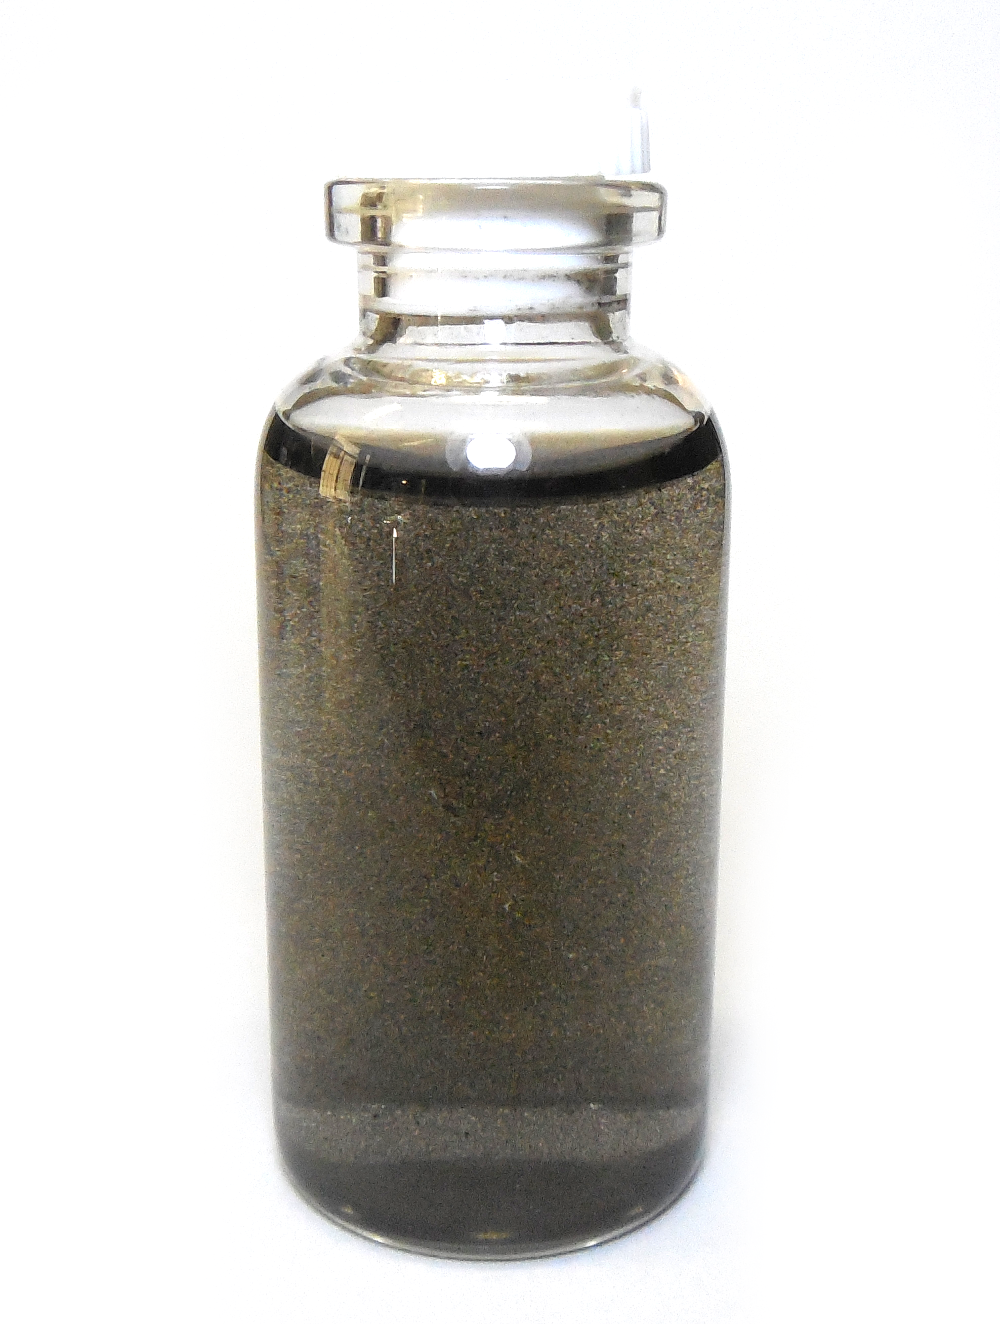
\includegraphics[width=\textwidth]{RGO_pic.png}
		\caption{RGO}
		\label{fig:RGO}
	\end{subfigure}
	\begin{subfigure}{0.42\textwidth}
		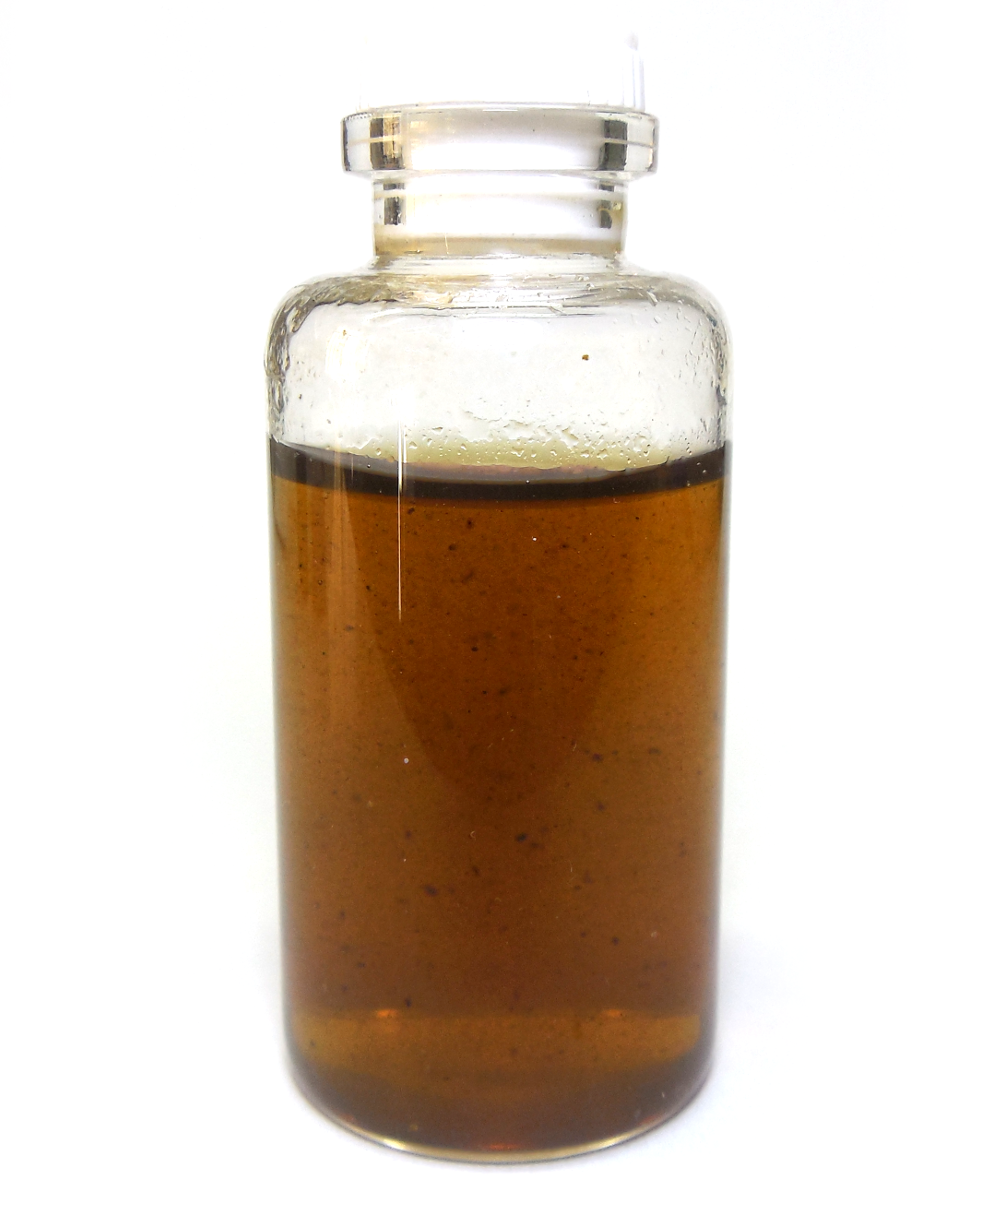
\includegraphics[width=\textwidth]{GO_pic.png}
		\caption{GO}
		\label{fig:GO}
	\end{subfigure}
	\caption{Muestras de rGO y GO en agua.}
\end{figure}


\begin{figure}
	\centering
	\begin{tikzpicture}[]
		\begin{axis}[
			cycle list name=colorbrewer-RYB,
			no markers,
			width = \textwidth,
			yticklabels={,,},
			ylabel={Intensidad [u.a.]},
			xlabel={2 $\theta$ [grados]},
			legend entries={Grafito, Óxido de grafeno, Óxido de grafeno reducido}]
			
			
			\addplot table [x expr = \thisrow{2t}, y expr=\thisrow{C}] {./Data/XRD/xrd.txt};
			\addplot table [x expr = \thisrow{2t}, y expr=\thisrow{GO}+1] {./Data/XRD/xrd.txt};
			\pgfplotsset{cycle list shift=1}
			\addplot table [x expr = \thisrow{2t}, y expr=\thisrow{RGO}+2] {./Data/XRD/xrd.txt};
%			\addplot table [x expr = \thisrow{2t}, y expr=\thisrow{RGOLYO}+3] {./Data/XRD/xrd.txt};
			\addplot +[mark=none, solid, black] coordinates {(10, 0) (10, 3)};
			\addplot +[mark=none, solid, black] coordinates {(23, 0) (23, 3)};
			\addplot +[mark=none, solid, black] coordinates {(26, 0) (26, 3)};
			\node[black, left] at (10, 3){\small{10\degree}};
			\node[black, left] at (23, 3){\small{23\degree}};
			\node[black, right] at (26, 3){\small{26\degree}};
		\end{axis}
	\end{tikzpicture}
	\caption{Espectro de difracción de rayos x.}
	\label{fig:xrd}
\end{figure}

\begin{figure}
	\centering
	\begin{subfigure}{\textwidth}
		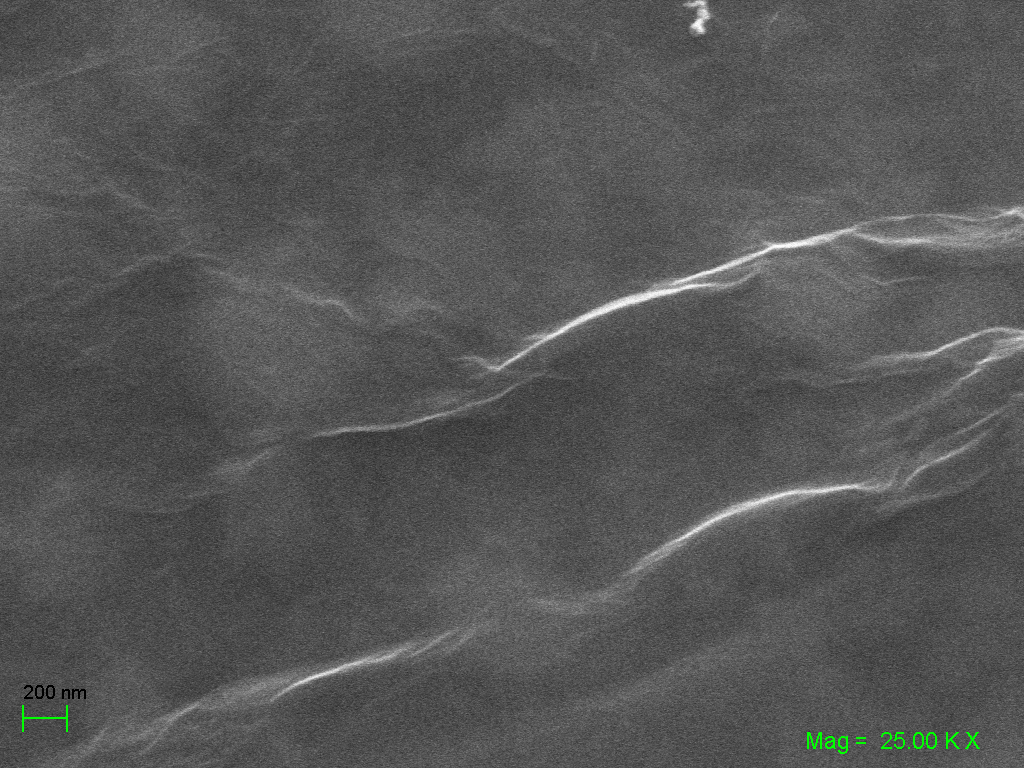
\includegraphics[width=\textwidth]{CRGO300517_paper.png}
	\end{subfigure}
	\begin{subfigure}{\textwidth}
		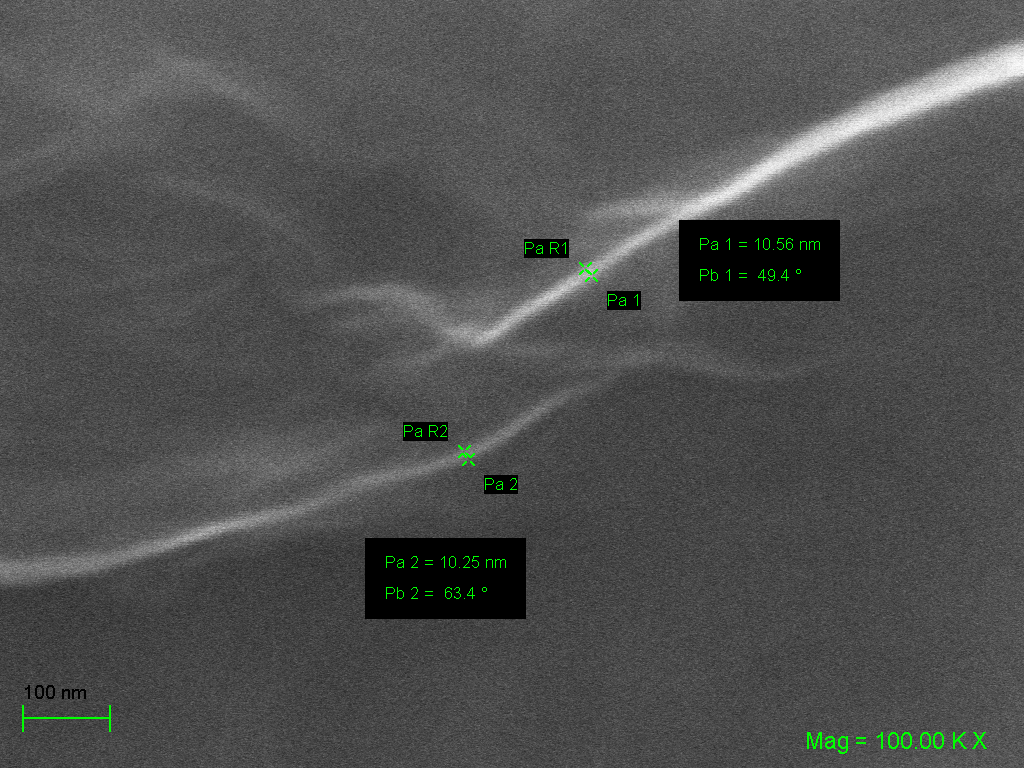
\includegraphics[width=\textwidth]{CRGO300517_paper_measures.png}
	\end{subfigure}
	\caption{text}
	\label{fig:rgo_paper_sem}
\end{figure}
